\documentclass[tikz,border=6pt]{standalone}
\usepackage[T1]{fontenc}
\usepackage{amsmath}
\usetikzlibrary{arrows.meta,positioning,calc}
\begin{document}
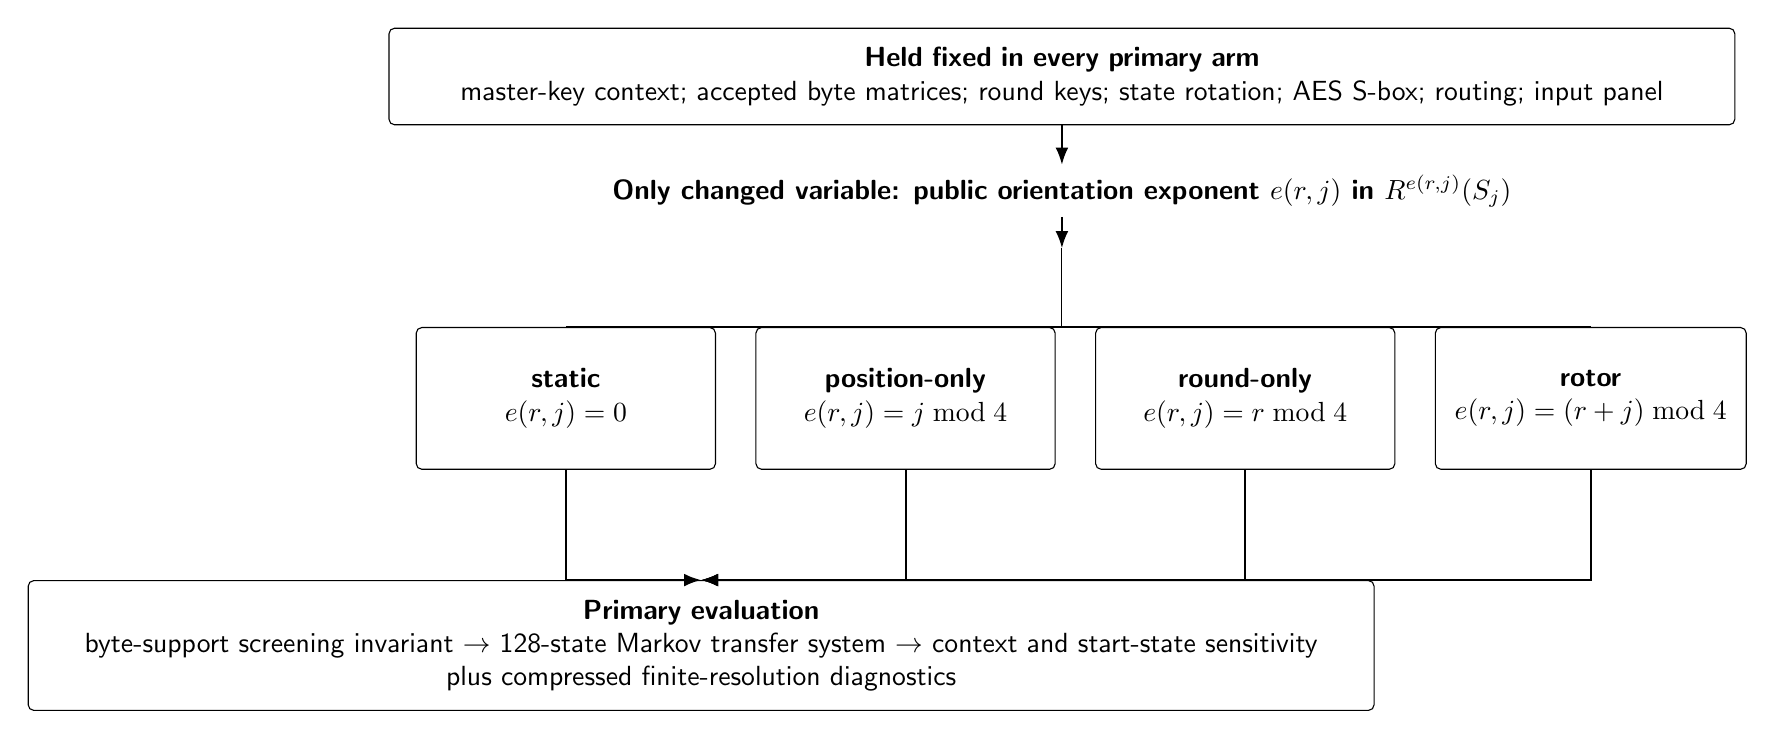
\begin{tikzpicture}[font=\sffamily\normalsize,>=Latex,
 fixed/.style={draw,rounded corners=2pt,align=center,inner sep=7pt,minimum height=12mm},
 arm/.style={draw,rounded corners=2pt,align=center,inner sep=7pt,minimum width=38mm,minimum height=18mm},
 arr/.style={->,line width=.7pt}]

\node[fixed,text width=166mm] (fixed) {\textbf{Held fixed in every primary arm}\\
master-key context; accepted byte matrices; round keys; state rotation; AES S-box; routing; input panel};

\node[below=5mm of fixed,font=\sffamily\bfseries] (varlabel) {Only changed variable: public orientation exponent $e(r,j)$ in $R^{e(r,j)}(S_j)$};

\node[arm,below=14mm of varlabel,xshift=-63mm] (st) {\textbf{static}\\$e(r,j)=0$};
\node[arm,right=5mm of st] (po) {\textbf{position-only}\\$e(r,j)=j\bmod4$};
\node[arm,right=5mm of po] (ro) {\textbf{round-only}\\$e(r,j)=r\bmod4$};
\node[arm,right=5mm of ro] (rot) {\textbf{rotor}\\$e(r,j)=(r+j)\bmod4$};

\coordinate (branch) at ($(varlabel.south)+(0,-4mm)$);
\draw[arr] (fixed.south) -- (varlabel.north);
\draw[arr] (varlabel.south) -- (branch);
\foreach \n in {st,po,ro,rot}{\draw (branch) |- (\n.north);}

\node[fixed,text width=166mm,below=14mm of po.south east,anchor=north east,xshift=40.5mm] (eval) {\textbf{Primary evaluation}\\
byte-support screening invariant $\rightarrow$ 128-state Markov transfer system $\rightarrow$ context and start-state sensitivity\\
plus compressed finite-resolution diagnostics};
\foreach \n in {st,po,ro,rot}{\draw[arr] (\n.south) -- ++(0,-4mm) |- (eval.north);}

\end{tikzpicture}
\end{document}
